% overleaf document: measured noise spectrum2 simulations with some small modifications. Also use passive voice instead of "we". 

This appenidx discusses the basic terminology of signal processing and gives the definitions which are used in this thesis. The focus is on Fourier transform and the power spectral density. First the most general mathematical definitions which concern signals continuous in time and with infinite time duration are discussed. Secondly, the definitions are given for signals sampled at a finite number of points, which are considered for the measurements and for the computational analysis. Furthermore, the quantities that are used most often for noise power spectrum measurements and their relationship to the mathematical definitions of the power spectral density are discussed. Finally, the way of applying a measured noise spectrum in numerical simulations is described.

\section{Continuous-time analysis}\label{app:continuous_time_analysis}
\subsubsection*{Fourier transform} %\hfill \break
A physical process (or signal or time series) can be described in the time domain by a continuous function of time, e.g.~$y(t)$, or else in the frequency domain, where the process is specified by giving its amplitude $\fourierxform{y}$ as a function of frequency, e.g.~$\fourierxform{y}(f)$ with $f \in \left(-\infty, +\infty \right )$. In other words, $y(t)$ and $\fourierxform{y}(f)$ are essentially different representations of the same function.  In general, $\fourierxform{y}(f)$ can be a complex quantity, with the complex argument giving the phase of the component at the frequency $f$.

One can switch between these two representations using the Fourier transform method. In this thesis the Fourier transform of a time series $y(t)$, which will be denoted in this document by $\fourierxform{y}$, is defined as~\cite{a_numerical_recipies}: %eq.12.0.1

\begin{equation}\label{eq:fft_definition}
\fourierxform{y}(f) = \int_{-\infty}^{\infty} y(t) e^{-2\pi \imagunit t f} dt,
\end{equation}
where $f$ stands for any real number. 
If the time is measured in seconds the frequency, $f$, is measured in hertz. 

The inverse Fourier transform, which is used to re-create the signal from its spectrum, is defined as:
\begin{equation}\label{eq:ifft_definition}
y(t) = \int_{-\infty}^{\infty} \fourierxform{y}(f) e^{2\pi \imagunit t f} df.
\end{equation}

\subsubsection*{Power spectral density and total power} %\hfill \break
The power spectral density, $S_{yy}(f)$, of a signal (or a time series), $y(t)$, will be used extensively in this thesis: it describes the distribution of the power in a signal between its frequency components, and is defined as the Fourier transform of the autocorrelation function, $R_{yy}(t)$~\cite{b_papoulis1991probability}: % Eq.10-14 p. 338

\begin{equation}\label{eq:Sxx_definition}
    S_{yy}(f) = \fourierxform{R}_{yy}(f) =  \int_{-\infty}^{\infty} R_{yy}(\tau)e^{-2\pi \imagunit \tau f} d\tau.
\end{equation}

The continuous autocorrelation $R_{yy}(\tau)$ is defined as the continuous cross-correlation integral of $y(t)$ with itself, at lag $\tau$~\cite{FFT_and_applications}:
\begin{equation}\label{eq:Rxx_definition}
    R_{yy}(\tau) = (y \ast y)(\tau) = \int_{-\infty}^{\infty} \bar{y}(t) y(t+\tau) dt,
\end{equation}
where $\ast$ denotes the convolution operation and $\bar{y}(t)$ represents the complex conjugate of $y(t)$.

% cross (lagged) correlation
According to the cross-correlation theorem \cite{FFT_and_applications}:
\begin{equation}\label{eq:cross_correlation_theorem}
\fourierxform{R}_{yy}(f) = \bar{\fourierxform{y}}(f) \fourierxform{y}(f) = \mid \fourierxform{y}(f) \mid ^2,
\end{equation}
where $\fourierxform{y}(f)$ is the Fourier transform of the signal as defined in Eq.~(\ref{eq:fft_definition}).

From Eq.~(\ref{eq:Sxx_definition}) and Eq.~(\ref{eq:cross_correlation_theorem}) the power spectral density of a signal $y(t)$ can be simply written as the square of its Fourier transform:
\begin{equation}\label{eq:Sxx_definition_v2}
S_{yy}(f) = \mid \fourierxform{y}(f) \mid ^2,
\end{equation}
with  $f \in \left(-\infty, +\infty \right )$.

\section{Discrete-time analysis}\label{app:discrete_time_analysis}

\subsubsection*{Discrete-time signals} %\hfill \break
% the following paragraph is from here: https://sceweb.sce.uhcl.edu/harman/ceng5431/2015WEB/Chap11tlhDFT.pdf
Figure~\ref{fig:sampling_of_continuous_signal} shows a part of a continuous signal $y(t)$. As already mentioned, for the measurements and the computational analysis, signals (or time series) sampled at a finite number of points are considered. Such signals are called discrete-time signals and in most cases they are sampled at equal points in time. For example, in Figure~\ref{fig:sampling_of_continuous_signal}, it is assumed that the continuous signal, $y(t)$, is sampled at intervals $\Delta t$ creating a set of $N$ points. The length in time between the first and final sample is $T_\mathrm{sample}=\frac{N-1}{N}T$, where $T = N\Delta t$. %One can see that the continuous signal is not only sampled but also truncated.


\begin{figure}[!ht]
     \centering         
     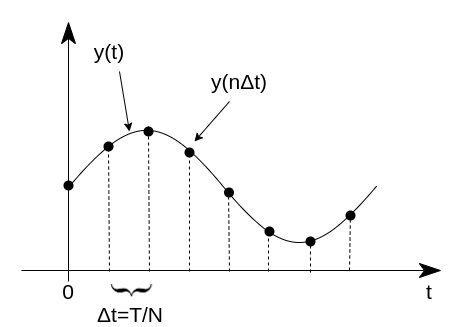
\includegraphics[width=0.5\textwidth]{./images/app_B/approximation_of_signal_by_sampling_v2.png}
         \caption{Sampling of the continuous signal $y(t)$ at a finite number of points $N$. The sampled signal is the discrete-time signal $y(n\Delta t)$ with $\Delta t$ the sampling interval and  $n$ an integer such that $n \in \left[0,N-1 \right ]$.}
         \label{fig:sampling_of_continuous_signal}
\end{figure}

\subsubsection*{Discrete Fourier transform} %\hfill \break %\label{subsec:DFT}
Let us consider a discrete-time signal, $y_n$ which is sampled at $N$ consecutive samples, $y_n = y(n \Delta t)$, with $n \in \left[0,N-1 \right ]$ such that $\Delta t$ is the sampling interval. For later convenience, we assume that $N$ is an odd integer. As a first step, we note that the integral of Eq.~(\ref{eq:fft_definition}) can be represented by a discrete sum in the limit that $\Delta t \to 0$:
\begin{equation}\label{eq:dft_proof}
\fourierxform{y}(f) = \int_{-\infty}^{\infty} y(t) e^{-2\pi \imagunit f t} dt =
\lim_{\Delta t \to 0}
\sum_{n=-\infty}^\infty y(n\Delta t) e^{-2\pi \imagunit f n \Delta t} \Delta t.
%= \Delta t \sum_{n=0}^{N-1} y(n\Delta t) e^{\frac{-j 2\pi k n}{N}},
\end{equation}
%where $f_k=k/(N\Delta t)$ and $k \in \left[-\frac{N-1}{2},+\frac{N-1}{2} \right ]$ (for odd $N$) or  $k \in \left[-\frac{N}{2},+\frac{N}{2} \right ]$ (for even $N$), and $k$ being an integer.

Based on the expression for the summation in Eq.~(\ref{eq:dft_proof}), we define the discrete Fourier transform as follows:
\begin{equation}\label{eq:DFT_definiton}
\fourierxform{y}_k= \sum_{n=0}^{N-1} y(n\Delta t) e^{-2\pi \imagunit \frac{k n}{N}}.
\end{equation}
Here, the index $k$ is an integer in the range $-\frac{N-1}{2}$ to $\frac{N-1}{2}$.
Each component $\fourierxform{y}_k$ of the discrete Fourier transform is related to the component $\fourierxform{y}(f)$ of the continuous Fourier transform of $y(t)$, for $f = k/T$, in the limit $\Delta t \to 0$ and $N \to \infty$ (and where it is assumed that $y(t) = 0$ for $t < 0$ and for $t > T$).

It should be noted that the discrete Fourier transform is calculated only at integer values of $k$, and therefore for $N$ samples the discrete Fourier transform will consist of $N$ numbers. The components of the discrete Fourier transform are calculated at frequencies $f_k$ that are integer multiples of $\Delta f = 1/T = f_s/N$, with $f_s = 1/\Delta t$ the sampling frequency. In that case, $f_k \in \left[-\frac{N-1}{2T},\frac{N-1}{2T} \right]$. An example of a discrete Fourier transform is shown in Fig.~\ref{fig:signal_and_DFT_example}.
%/Delta_f is the resolution frequency
\begin{figure}[!ht]
    \centering
    \begin{subfigure}[t]{0.45\textwidth}
        \centering
        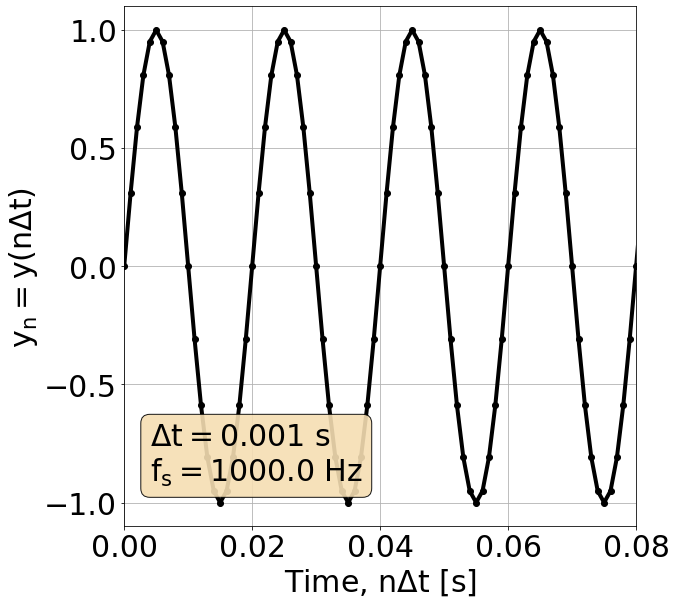
\includegraphics[width=1\textwidth]{./images/app_B/simple_signal_1freq_example.png}
        \caption{$y=\sin(2 \pi f t),\ f=50$ Hz}
        \label{fig:signal_and_DFT_example_a}
    \end{subfigure}
    \hfill
    \begin{subfigure}[t]{0.45\textwidth}
        \centering
        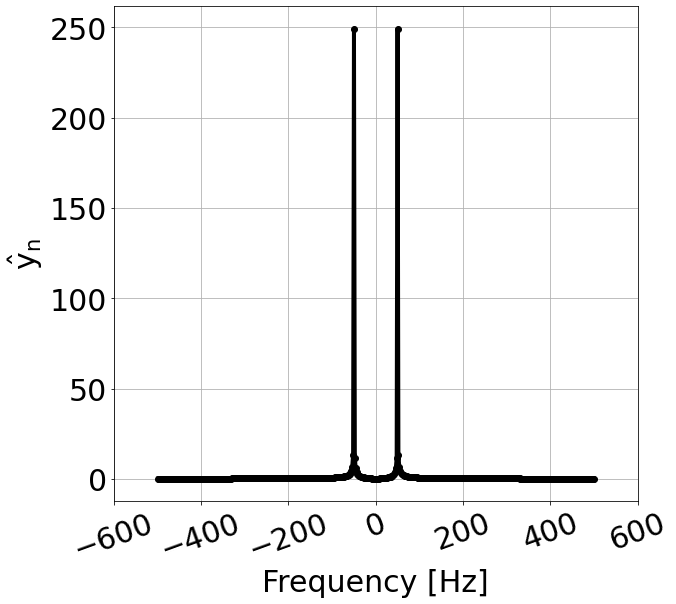
\includegraphics[width=1\textwidth]{./images/app_B/simple_signal_1freq_fft_example.png}
        \caption{Discrete Fourier transform}
        \label{fig:signal_and_DFT_example_b}
    \end{subfigure}
    \hfill
     \caption{Example of a signal sampled at discrete time intervals, and the corresponding discrete Fourier transform.}
     \label{fig:signal_and_DFT_example}
\end{figure}

The inverse discrete Fourier transform is defined as:
\begin{equation}\label{eq:iDFT_definiton}
 y_n =  y(n\Delta t) = \frac{1}{N} \sum_{k=-\frac{N-1}{2}}^{\frac{N-1}{2}} \fourierxform{y}_k e^{2\pi \imagunit \frac{k n}{N}},
\end{equation}
where $n \in \left[0,N-1 \right ]$ and where $n$ and $k$ are both integers.

The definitions given in Eq.~(\ref{eq:DFT_definiton}) and Eq.~(\ref{eq:iDFT_definiton}) are consistent with those used in numpy, in the numpy.fft function \cite{numpy_fft} package of the Python programming language. 

\subsubsection*{Power spectral density} % \hfill \break
Following Eq.~(\ref{eq:Sxx_definition_v2}) the power spectral density of a discrete-time signal should be estimated as follows:

\begin{equation}\label{eq:Sxx_definition_discrete_not_normalised}
    S_{yy}(f_k) = A \mid \fourierxform{y}_k(f_k) \mid ^2,
\end{equation}
where $f_k \in \left[-\frac{N-1}{2T},\frac{N-1}{2T} \right]$. $A$ is a normalisation constant which is introduced in order to obtain the correct amplitudes at each frequency and thus the correct noise power. There are several different conventions for the choice of this normalization. In this thesis, the following normalization is considered (see more details in the dedicated paragraph at the end of this section):
\begin{equation}\label{eq:Sxx_definition_discrete_normalized}
    S_{yy}(f_k) = \frac{1}{N^2 \Delta f} \mid \fourierxform{y}_k(f_k) \mid ^2,
\end{equation}
where  $\Delta f = 1/T$ the frequency resolution and $N$ the number of samples.
    
\begin{figure}[!ht]
    \centering         
    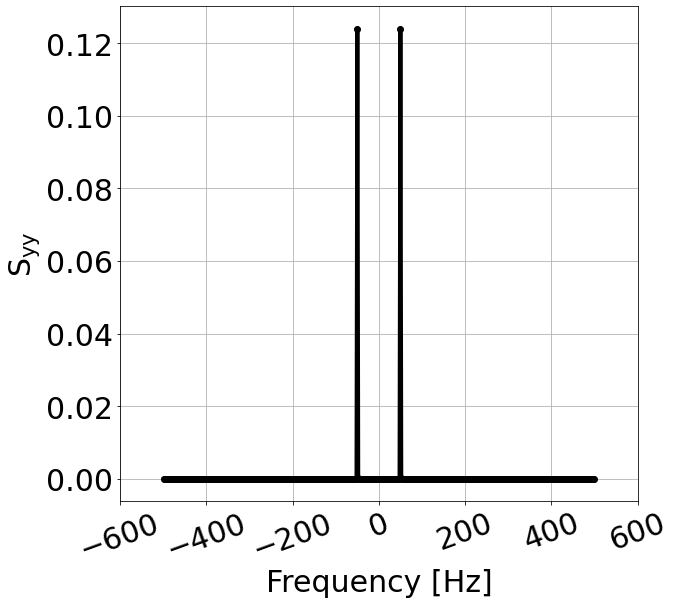
\includegraphics[width=0.5\textwidth]{./images/app_B/simple_signal_1freq_psd_example.png}
        \caption{Power spectrum of $y=\sin(2 \pi f t),\ f = $50\,Hz.}
        \label{fig:psd_example_two_sided}
\end{figure}

Figure~\ref{fig:psd_example_two_sided} shows an example power spectrum of the time-domain signal shown in Fig.~\ref{fig:signal_and_DFT_example}a. It can be seen that the spectrum that results from the analysis above is two-sided, which means that it has both positive and negative frequencies. It is also symmetric around the DC component ($f = $0\,Hz), which is actually a property of a real signal. 

The power spectral density is expressed in terms of the square of the amplitude of the signal per unit frequency. For example, for a signal defined in units of voltage, V, (e.g. from an oscillator) the units are $\mathrm{V^2/Hz}$.

\subsubsection*{Conversion of a two-sided power spectrum to a single-sided power spectrum} %\hfill \break
% From https://www.sjsu.edu/people/burford.furman/docs/me120/FFT_tutorial_NI.pdf. Rephrase
As already mentioned, the frequency spectrum of a real signal is symmetric around the DC component and therefore the information contained in the negative frequency is redundant. For this reason, most of the instruments used in experiments to display a frequency analysis show just the positive part of the spectrum (single-sided spectrum).  

In order to convert from a two-sided spectrum to a single-sided spectrum, the negative part of the spectrum is discarded, and the amplitudes of the positive frequency components (excluding the DC component, so for $f > 0$) are multiplied by a factor 2:
\begin{equation}\label{eq:two-sided_2_single-sided}
        G_{yy}(f_k) = \left\{\begin{matrix}
  0, & f_k < 0 \\ 
    S_{yy}(f_k), & f_k=0  \\
     2 S_{yy}(f_k), & f_k > 0 
    \end{matrix}\right.
\end{equation}
where $S_{yy}(f_k)$ is the two-sided spectrum and $G_{yy}(f_k)$ the single-sided spectrum. Figure~\ref{fig:psd_example_single_sided} illustrates the single-sided spectrum of the signal shown in Fig.~\ref{fig:signal_and_DFT_example_a}.

\begin{figure}[!ht]
    \centering         
    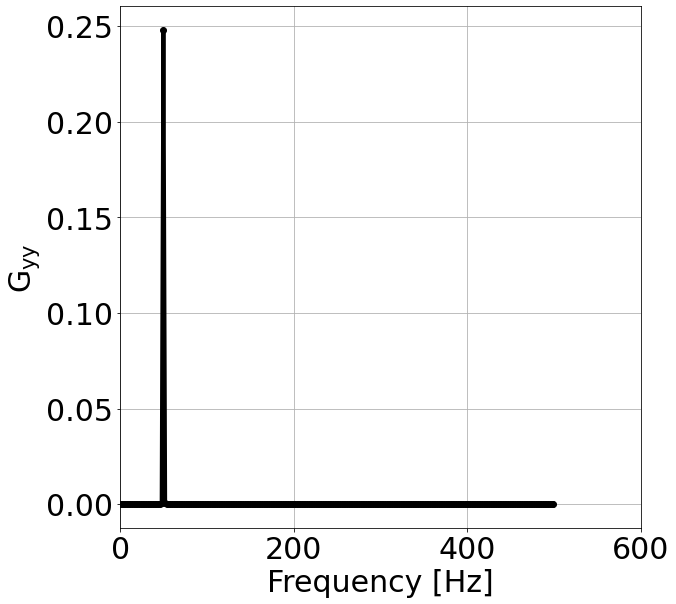
\includegraphics[width=0.5\textwidth]{./images/app_B/simple_signal_1freq_psd_single_sided_example.png}
        \caption{Single-sided power spectrum of the signal shown in Fig.~\ref{fig:signal_and_DFT_example}(a).}
        \label{fig:psd_example_single_sided}
\end{figure}

\subsubsection*{Normalisation factor for the power spectral density of a discrete-time signal}\label{appendix_dft_normalisation}
This paragraph, discusses the choice of the normalisation factor $A=1/(N^2 \Delta f)$ for the power spectral density of a discrete-time signal defined in Eq.~\eqref{eq:Sxx_definition_discrete_not_normalised}:
\begin{equation}
S_{yy}(f_k) = A \mid \fourierxform{y}_k(f_k) \mid ^2.
\end{equation}

Consider the example of a discrete-time series $y_n = y(n\Delta t)$ where $n$ is an integer such that $n \in [0, N-1]$. $y_n$ represents a sequence of successive points equally spaced in time, drawn from a normal distribution with known standard deviation $\sigma$ and zero mean, $\mu=0$. The variance of this collection of $N$ equally spaced values is given by:
\begin{equation}\label{eq:variance}
    \sigma^2 = \frac{1}{N}\sum_{n=0}^{N-1} \left | y_n \right |^2.
\end{equation}
According to Parseval's theorem~\cite{FFT_and_applications}, the variance can be written as:
%p.112
\begin{equation}\label{eq:variance_2}
    \sigma^2 = \frac{1}{N^2}\sum_{k=-\frac{N-1}{2}}^{\frac{N-1}{2}} \left | \fourierxform{y}_k \right |^2,
\end{equation}
where $\fourierxform{y}_k$ is the discrete Fourier transform of $y_n$.

Using Eq.~(\ref{eq:Sxx_definition}), the autocorrelation function $R_{yy}(\tau)$ for a continuous-time signal can be found from the inverse Fourier transform of $S_{yy}(f)$:
\begin{equation}\label{eq:autocorrelation_ivnerse}
R_{yy}(\tau) = \int_{-\infty}^{\infty} \bar{y}(t) y(t+\tau) \, dt = \int_{-\infty}^{\infty} S_{yy}(f) e^{2\pi \imagunit t f} \, df.
\end{equation}
For zero lag, this becomes:
\begin{equation}\label{eq:autocorrelation_zero_lag}
R_{yy}(0) = \int_{-\infty}^{\infty} S_{yy}(f) \, df = \sigma^2.
\end{equation}
This expresses the fact that the autocorrelation of a zero-mean stochastic process (such as $y_n$) is equal to the variance. It should be noted here that this integration over the spectral components yields the total power of the process.

For a discrete-time signal, we require that the power spectral density $S_{yy}(f_k)$ corresponds to the power spectral density for the continuous-time signal. In that case, Eq.~\eqref{eq:autocorrelation_zero_lag}
becomes:
\begin{equation}\label{eq:autocorrelation_zero_lag_discrete}
\sigma^2 =  \sum_{k=-\frac{N-1}{2}}^{\frac{N-1}{2}} S_{yy}(f_k) \Delta f.
\end{equation}

From Eq.~(\ref{eq:variance_2}) and Eq.~(\ref{eq:autocorrelation_zero_lag_discrete}) this leads to:
\begin{equation}\label{eq:normalisation_test}
 \frac{1}{N^2}\sum_{k=-\frac{N-1}{2}}^{\frac{N-1}{2}} \left | \fourierxform{y}_k \right |^2 =  \sum_{k=-\frac{N-1}{2}}^{\frac{N-1}{2}} S_{yy}(f_k) \Delta f,
\end{equation} %\Rightarrow \\
and hence:
\begin{equation}
  \sum_{k=-\frac{N-1}{2}}^{\frac{N-1}{2}} \frac{\left | \fourierxform{y}_k \right |^2}{N^2 \Delta f} =  \sum_{k=-\frac{N-1}{2}}^{\frac{N-1}{2}} S_{yy}(f_k).
\end{equation}
Therefore, to satisfy the requirement that the power spectral density for the discrete-time signal corresponds to that for the continuous-time signal, we define the power spectral density for a discrete-time signal:
\begin{equation}
    S_{yy}(f_k) = \frac{\left | \fourierxform{y}_k \right |^2}{N^2 \Delta f}.
\end{equation}
Hence, the normalisation factor in Eq.~\eqref{eq:Sxx_definition_discrete_not_normalised} is chosen to be:
\begin{equation}
    A=\frac{1}{N^2 \Delta f}.
\end{equation}


\section{Measuring amplitude and phase noise}\label{subsec:Measure_noise}

Amplitude and phase modulation are two of the main types of noise in the output signal of an oscillator. The instantaneous output voltage of an ideal oscillator can be expressed as:
\begin{equation}
    V(t) = V_0 \sin(2\pi f_0 t),
\end{equation}
where $V_0$ is the nominal peak voltage amplitude and $f_0$ the nominal frequency. 

However, in practice, small inaccuracies will introduce amplitude and phase modulations. These modulations are included in the above signal by adding stochastic processes, represented by $\phi(t)$ and $\epsilon (t)$, as follows:
\begin{equation}\label{eq:Oscillator_PN_AN}
    \begin{split}
    V(t) = &~(V_0+\epsilon(t)) \sin(2\pi f_0 t + \phi(t)), \\
    = &~\left( 1+\frac{\epsilon(t)}{V_0} \right) V_0 \sin(2\pi f_0 t + \phi(t)), \\ =  &~(1+\alpha(t)) V_0 \sin(2\pi f_0 t + \phi(t)),
    \end{split}
\end{equation}
where $\phi(t)$ is the deviation from the nominal phase $2\pi f_0 t$, $\epsilon(t)$ is the deviation from the nominal amplitude and $\alpha(t)=\epsilon(t)/V_0$ is the normalised amplitude deviation.  An example of a signal with phase and amplitude noise is shown in Fig.~\ref{fig:AN_PN_example}. 

\begin{figure}[!ht]
    \centering
    \begin{subfigure}[b]{0.45\textwidth}
        \centering
        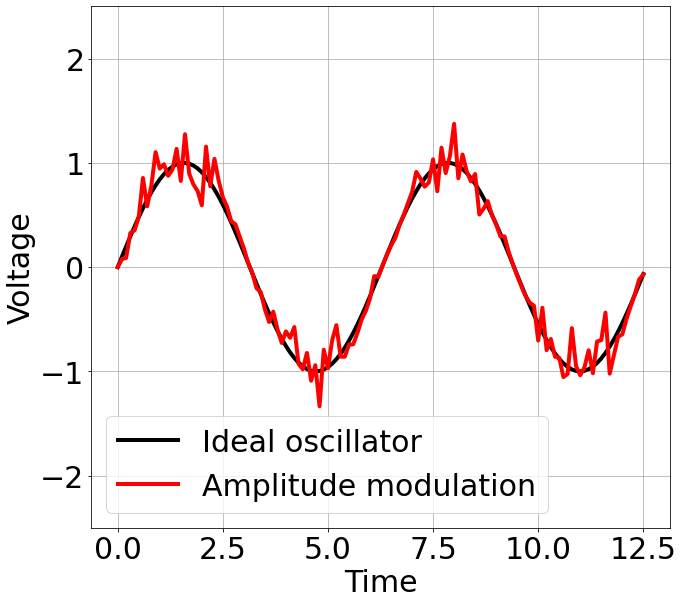
\includegraphics[width=1\textwidth]{./images/app_B/oscillator_example_AN.png}
        \caption{Amplitude noise}
        \label{fig:AN_PN_example_a}
    \end{subfigure}
    \hfill
    \begin{subfigure}[b]{0.45 \textwidth}
        \centering
        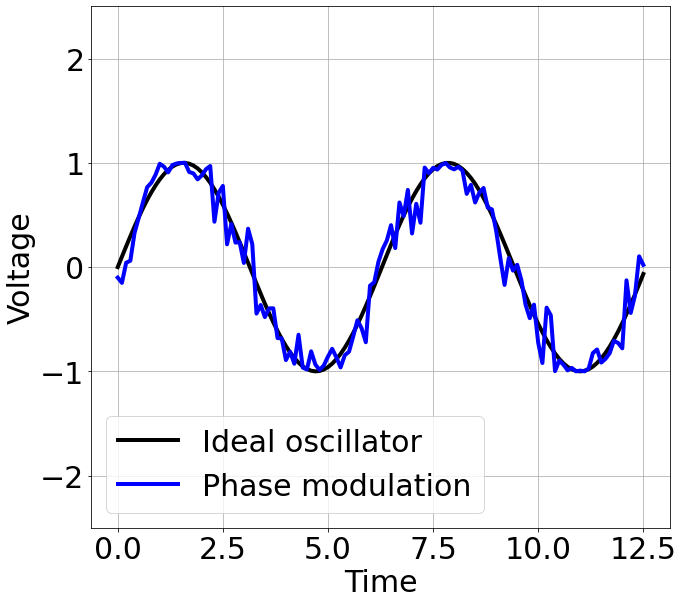
\includegraphics[width=1 \textwidth]{./images/app_B/oscillator_example_PN.png}
        \caption{Phase noise}
        \label{fig:AN_PN_example_b}
    \end{subfigure}
    \hfill
    \begin{subfigure}[b]{0.45\textwidth}
        \centering
        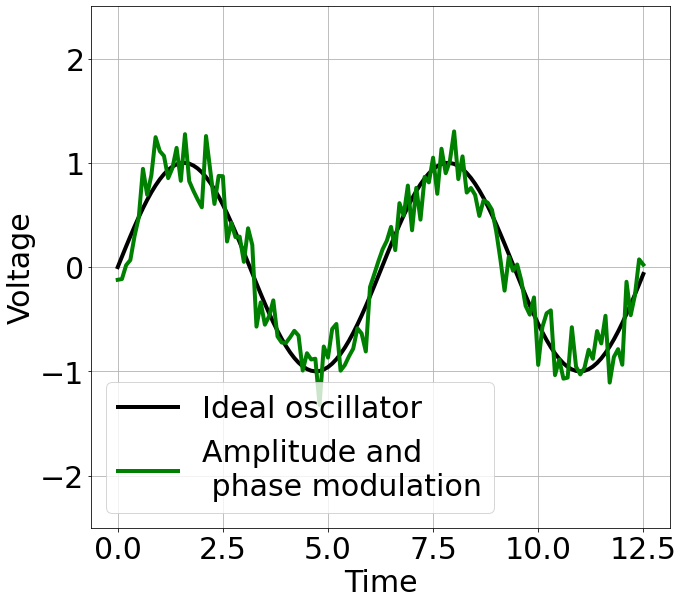
\includegraphics[width=1\textwidth]{./images/app_B/oscillator_example_AN_PN.png}
        \caption{Amplitude and phase noise}
        \label{fig:AN_PN_example_c}
    \end{subfigure}
    \hfill
    \caption{Instantaneous voltage of an oscillator in the presence of (a) amplitude noise, (b) phase noise, and (c) both amplitude and phase noise.}
    \label{fig:AN_PN_example}
\end{figure}